\paragraph{}
We are going to use min-cut algorithm. For this we construct the following graph (see Fig. \ref{fig:Diagramme2}) :
\paragraph{Vertices}
\begin{itemize}
\item a source S
\item a sink T
\item n vertices called $F_1,...,F_n$
\end{itemize}

\paragraph{Edges}
\begin{itemize}
\item n edges from S to $F_i$ with capacity $b_i$
\item n edges from $F_i$ to T with capacity $a_i$
\item n x (n-1) / 2 edges from $F_i$ to $F_j$ with capacity $c_{ij}$
\end{itemize}

\begin{figure}[h]
	\centering
		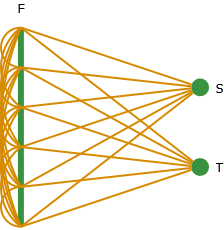
\includegraphics[width=6cm]{Diagramme2.png}
	\caption{Green = Vertices; Yellow = Edges}
	\label{fig:Diagramme2}
\end{figure}

\paragraph{}
We then realize that the capacity of a cut in this graph corresponds to the yearly cost of building firms linked to the source in town A and firms linked to the sink in town B. We conclude that min-cut algorithm gives an optimal repartition of the firms.

\paragraph{}
Furthermore our algorithm is polynomial, because the size of the graph is a linear function of the size of the input and Min-Cut is polynomial.